%-----------------------------------------------------------------------
% Beginning of chap2.tex
%-----------------------------------------------------------------------
%
%  AMS-LaTeX sample file for a chapter of a monograph, to be used with
%  an AMS monograph document class.  This is a data file input by
%  chapter.tex.
%
%  Use this file as a model for a chapter; DO NOT START BY removing its
%  contents and filling in your own text.
% 
%%%%%%%%%%%%%%%%%%%%%%%%%%%%%%%%%%%%%%%%%%%%%%%%%%%%%%%%%%%%%%%%%%%%%%%%


\chapter*{Lecture 3}
\addcontentsline{toc}{chapter}{Lecture 3}
\addtocounter{chapter}{1}
\addtocounter{section}{-2}
%\numberwithin{section}{chapter}
\numberwithin{equation}{chapter}
\numberwithin{theorem}{chapter}
% \epigraph{}{--- \textup{}}

Most modern optimization methods are iterative: they generate a sequence of points $\vct{x}_0,\vct{x}_1,\dots$ in $\R^d$
in the hope that this sequences will converge to a local or global minimizer $\vct{x}^*$ of a function $f(\vct{x})$. A typical rule for generating such a sequence would be to start with a vector $\vct{x}_0$, chosen by an educated guess, and then for $k\geq 0$, move from step $k$ to $k+1$ by
\begin{equation*}
 \vct{x}_{k+1} = \vct{x}_k+\alpha_k\vct{p}_k,
\end{equation*}
in a way that ensures that $f(\vct{x}_{k+1})\leq f(\vct{x}_k)$.
The parameter $\alpha_k$ is called the {\em step length}, while $\vct{p}_k$ is the {\em search direction}. In this lecture we discuss one such method, the method of Gradient descent, or steepest descent.

\section{Gradient descent} In the method of gradient descent, the search direction is chosen as
\begin{equation}\label{eq:gradient}
 \vct{p}_k = -\nabla f(\vct{x}_k).
\end{equation}
To see why this makes sense, let $\vct{p}$ be a direction with $\norm{\vct{p}}_2=1$ and consider the Taylor expansion
\begin{equation*}
 f(\vct{x}_k+\alpha \vct{p}) = f(\vct{x}_k)+\alpha \ip{\vct{p}}{\nabla f(\vct{x}_k)}+O(\alpha^2).
\end{equation*}
Considering this as a function of $\alpha$, the rate of change in direction $\vct{p}$ at $\vct{x}_k$ is the derivative of this function at $\alpha=0$,
\begin{equation*}
 \frac{df(\vct{x}_k+\alpha \vct{p})}{d\alpha}|_{\alpha=0} = \ip{\vct{p}}{\nabla f(\vct{x}_k)},
\end{equation*}
also known as the {\em directional derivative} of $f$ in the direction $\vct{p}$.
This formula indicates that the rate of change is {\em negative}, and we have a {\em descent direction}, if $\ip{\vct{p}}{\nabla f(\vct{x}_k)}<0$. The Cauchy-Schwarz inequality gives the bounds
\begin{equation*}
 -\norm{\vct{p}}_2 \norm{\nabla f(\vct{x}_k)}_2 \leq \ip{\vct{p}}{\nabla f(\vct{x}_k)} \leq \norm{\vct{p}}_2 \norm{\nabla f(\vct{x}_k)}_2.
\end{equation*}
We see that the rate of change is the smallest when the first inequality is an equality, which happens if 
\begin{equation*}
 \vct{p} = -\frac{\nabla f(\vct{x}_k)}{\norm{\nabla f(\vct{x}_k)}}_2.
\end{equation*}
In making a step $\vct{x}_{k+1}=\vct{x}_k+\alpha_k\vct{p}_k$, the part of $\vct{p}_k$ that is of interest is only the direction, not the size: the latter can be adjusted using the step length parameter $\alpha_k$. We can therefore choose $\vct{p}_k$ as in~\eqref{eq:gradient} as the direction of steepest descent.

\subsection{Step length selection}
The step length can then be chosen as the minimizer of the function
\begin{equation*}
 \alpha \mapsto \oldphi(\alpha) := f(\vct{x}_k-\alpha \nabla f(\vct{x}_k)).
\end{equation*}
In practice minimizing this function is not always the most efficient (or even possible) thing to do. One would rather choose a step length that satisfies some criteria that ensure that the sequence $\vct{x}_k$ converges to a minimizer $\vct{x}^*$ under suitable conditions on a function $f$. One such set of conditions are the Armijo-Goldstein conditions, which state that a step length $\alpha$ should satisfy 
\begin{equation}\label{eq:armgold}
 \oldphi(0)+(1-c)\cdot \alpha \cdot \oldphi'(0)\leq \oldphi(\alpha) \leq \oldphi(0)+c\cdot \alpha \cdot \oldphi'(0).
\end{equation}
for a constant $c\in (0,1/2)$ (typically of order $10^{-4}$). Note that
\begin{equation*}
 \phi(0) = f(\vct{x}_k), \quad \phi(\alpha) = f(\vct{x}_k-\alpha\nabla f(\vct{x}_k)), \quad \phi'(0) = -\norm{\nabla f(\vct{x}_k)}_2^2,
\end{equation*}
so that the inequalities~\eqref{eq:armgold} can be written equivalently (after some rearranging) as
\begin{equation*}
 c\alpha \norm{\nabla f(\vct{x}_k)}_2^2 \leq f(\vct{x}_k)-f(\vct{x}_k-\alpha \nabla f(\vct{x}_k)) \leq (1-c)\alpha \norm{\nabla f(\vct{x}_k)}_2^2
\end{equation*}

We explain these inequalities.

\begin{enumerate}
\item The right bound in~\eqref{eq:armgold} is a {\em sufficient decrease condition}: it ensures that $f(\vct{x}_{k+1})$ not only decreases, but decreases enough to converge to a local minimum. To see why this condition is necessary, consider the function $f(x)=x^2-1$ and the sequence $x_k = \sqrt{1+1/k}$ for $k\geq 1$. Clearly, the sequence $f(\vct{x}_k)=1/k$ decreases, but fails to converge to the minimizer $f(0)=-1$.
\item As the right bound can always be satisfied when $\alpha$ is small enough, the left-hand side is there to ensure that the step-length is not too short. A popular alternative is to replace the left-hand side by the {\em curvature condition} $\oldphi'(\alpha)\geq \tilde{c} \oldphi'(0)$ for some $\tilde{c}\in (c,1)$, leading to what is know as the Wolfe conditions, but we will not discuss these at this point.
\end{enumerate}

\begin{example}
 Consider the function $f\colon \R^2\to \R$ defined by $f(\vct{x}) = x_1^2+x_2^2$. The gradient is $\nabla f(\vct{x}) = 2\vct{x}$, and the $\phi$ function at $\vct{x}_k=(1,1)^{\trans}$
 \begin{equation*}
  \phi(\alpha) = f(\vct{x}_k-\alpha \nabla f(\vct{x}_k)) = 2(1-2\alpha)^2, \quad \phi'(\alpha) = -8(1-2\alpha).
 \end{equation*}
The Armijo-Goldstein conditions~\eqref{eq:armgold} then state that we can choose $\alpha$ such that
\begin{equation*}
 2(1-4(1-c)\alpha) \leq 2(1-2\alpha)^2 \leq 2(1-4c\alpha).
\end{equation*}
For the choice $c=1/4$, the valid interval is part of the $x$-axis delimited by the vertical lines in Figure~\ref{fig:armgold}. The optimal step length in this case would be $\alpha=0.5$.

\begin{figure}[h!]\label{fig:armgold}
\centering
 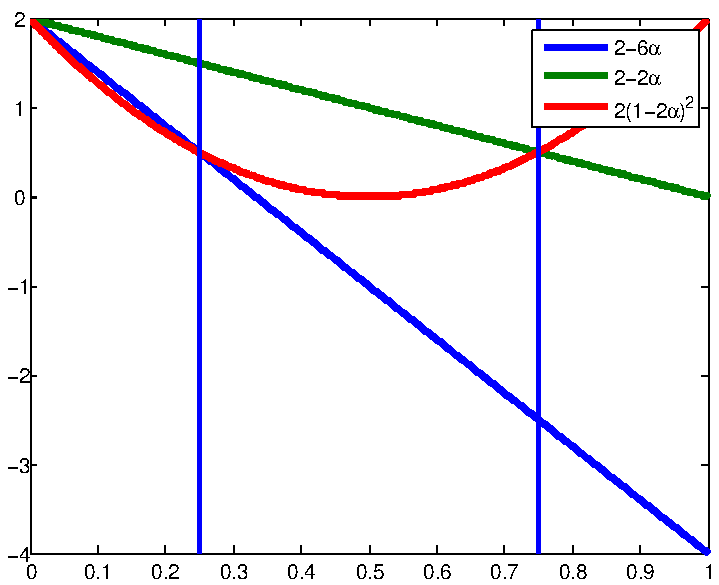
\includegraphics[width=0.5\textwidth]{images/goldarmijo_cropped.pdf}
 \caption{Choosing a step length.}
\end{figure}

\end{example}

\subsection{Linear least squares} An important special case is when the function has the form
\begin{equation*}
 f(\vct{x}) = \frac{1}{2}\norm{\mtx{A}\vct{x}-\vct{b}}_2^2.
\end{equation*}
Recall from Problem (1.5) that the Hessian is symmetric and positive semidefinite, with the gradient given by
\begin{equation*}
 \nabla f(\vct{x}) = \mtx{A}^{\trans}(\mtx{A}\vct{x}-\vct{b}).
\end{equation*}
The method of gradient descent proceeds as
\begin{equation*}
 \vct{x}_{k+1} = \vct{x}_k-\alpha_k \mtx{A}^{\top}(\mtx{A}\vct{x}_k-\vct{b}).
\end{equation*}
To find the best $\alpha_k$, we compute the minimum of the function
\begin{equation}\label{eq:minalpha}
 \alpha \mapsto f(\vct{x}+\alpha \mtx{A}^{\trans}(\vct{b}-\mtx{A}\vct{x})).
\end{equation}
If we set $\vct{r}:=\mtx{A}^{\trans}(\vct{b}-\mtx{A}\vct{x})$ and compute the minimum of~\eqref{eq:minalpha} by differentiating, we get the step length
\begin{equation*}
 \alpha = \frac{\vct{r}^{\trans}\vct{r}}{\vct{r}^{\trans}\mtx{A}^\trans\mtx{A}\vct{r}}.
\end{equation*}
The gradient descent algorithm for the linear least squares problem proceeds by first computing $\vct{r}_0=\mtx{A}^{\trans}(\vct{b}-\mtx{A}\vct{x}_0)$, and then at each step
\begin{align*}
 \alpha_k &= \frac{\vct{r}_k^{\trans}\vct{r}_k}{\vct{r}_k^{\trans}\mtx{A}^\trans\mtx{A}\vct{r}_k}\\
 \vct{x}_{k+1} &= \vct{x}_k+\alpha_k \vct{r}_k\\
 \vct{r}_{k+1} &= \vct{r}_k - \alpha_{k}\mtx{A}^{\trans}\mtx{A}\vct{r}_k.
\end{align*}
Does this work? How do we know when to stop? It is worth noting that the residual satisfies $\vct{r}=0$ if and only if $\vct{x}$ is a stationary point, in our case, a minimizer. One criteria for stopping could then be to check whether $\norm{\vct{r}_k}_2\leq \e$ for some given tolerance $\e>0$.

\begin{example}
 We test this method with the linear regression problem from Lecture 1, where we determinded the relationship $Y=\beta_0+\beta_1X$ of adult mass to basal metabolic rate in mammals. In this example, the matrix $\mtx{A}$ is the $2\times 573$ matrix
 \begin{equation*}
  \mtx{A} = \begin{pmatrix}
             1 & x_1\\
             \vdots & \vdots\\
             1 & x_{573}
            \end{pmatrix},
            \end{equation*}
where the $x_i$ represent the mass of mammal $i$, and the vector $\vct{b}$ consists of the metabolic rate parameters. The $2$-vector $\vct{x}$ represents the two values $\beta_0$ and $\beta_1$. A naive MATLAB code for gradient descent looks as follows.
\begin{lstlisting}
function xout = graddesc(A,b,x,tol)
    r = A'*(b-A*x);
    while norm(r,2)>tol
        Ar = A*r;
        alpha = r'*r/(Ar'*Ar);
        x = x+alpha*r;
        r = r-alpha*A'*Ar;
    end
    xout = x;
end
\end{lstlisting}
The result is the same as when using the MATLAB solver or CVX,
$\beta_0 = 1.36$, $\beta_1 = 0.70$.
\end{example}


In the next lecture we will introduce the concept of rate of convergence and analyse the rate of convergence of gradient descent.

%-----------------------------------------------------------------------
% End of chap1.tex
%-----------------------------------------------------------------------
